\documentclass{article}
\usepackage{graphicx}
\title{A proposal for the development of the networking device  for implementation of  private 5G networks}
\author{Madhav Desai, D. Manjunath, L. Somappa, Gaurav Kasbekar\\ IIT Bombay\\ Abhijit Chaudhary \\ Niral Networks}
\begin{document}
\maketitle

\section{Aims and Objective of the Project}

	The aim of the project is to build a trusted hardware platform
	which can be configured to form the core of a private 5G network.

	Networked devices, and devices that connect to other computing devices are 
	vulnerable to tampering and malicious compromise through both their software and hardware. 

	In our proposal, we will build a trusted hardware platform around 
	a core technology of the AJIT multi-threaded multi-core processor.   
	This processor has been developed at IIT Bombay, and has been used 
	successfully in the implementation of an IRNSS + GPS
	base-band receiver system.   Innovations such as route caching and packet
	flow interpreters will be integrated into the fabric of the proposed hardware
	platform.

	Further, the trusted hardware will run software which is completely open
	to user inspection and oversight.   The software is based on open source
	computations and will be ported to the hardware platform.


\section{Novelty of the proposed project}

	The novelty of the project can be summarized in three ways
	
	\begin{itemize}
	\item Trust:
		The key elements in establishing trust are: 
		\begin{itemize}
			\item the identity of the developer institution and personnel, in this case led
			by IIT-Bombay.

			\item the transparency and documentation of the technology.
		\end{itemize}
	\item Made in India:
		Implies control over technology, longevity of the technology,
		cost advantages, independence and spin-offs.

	\item Non-proprietary software:
		Completely auditable, based on open standards, and with source
		code completely visible and shared.
	\end{itemize}

	With that background, we propose a program of developing and deploying  private 5G subsystems.
	Our target deployment is the critical national infrastructure such as military establishments, 
	power grids, refineries, railways, shipyards, ordnance and armament factories, etc. 

	The hardware for such systems will be based on the work at IIT Bombay. The software will be from 
	Niral Networks who have been developing software-based communication systems.


\section{Detailed Description of the project: hardware platform}

	The project involves the development of a hardware network router using the
	AJIT multi-threaded multi-core processor, and the porting and customization of
	software from Niral Networks on to this router. 

	The hardware network router will be built using a multi-threaded multi-core
	64-bit AJIT processor, with four cores and eight threads.  The hardware
	router will be constructed in three phases over an 18 month period.

\subsection{Phase 1}

	In phase 1, a basic router which integrates the multi-core processor with
	four network interfaces will be built (See Figure \ref{fig:Phase1}):

\begin{figure}
  \centering
  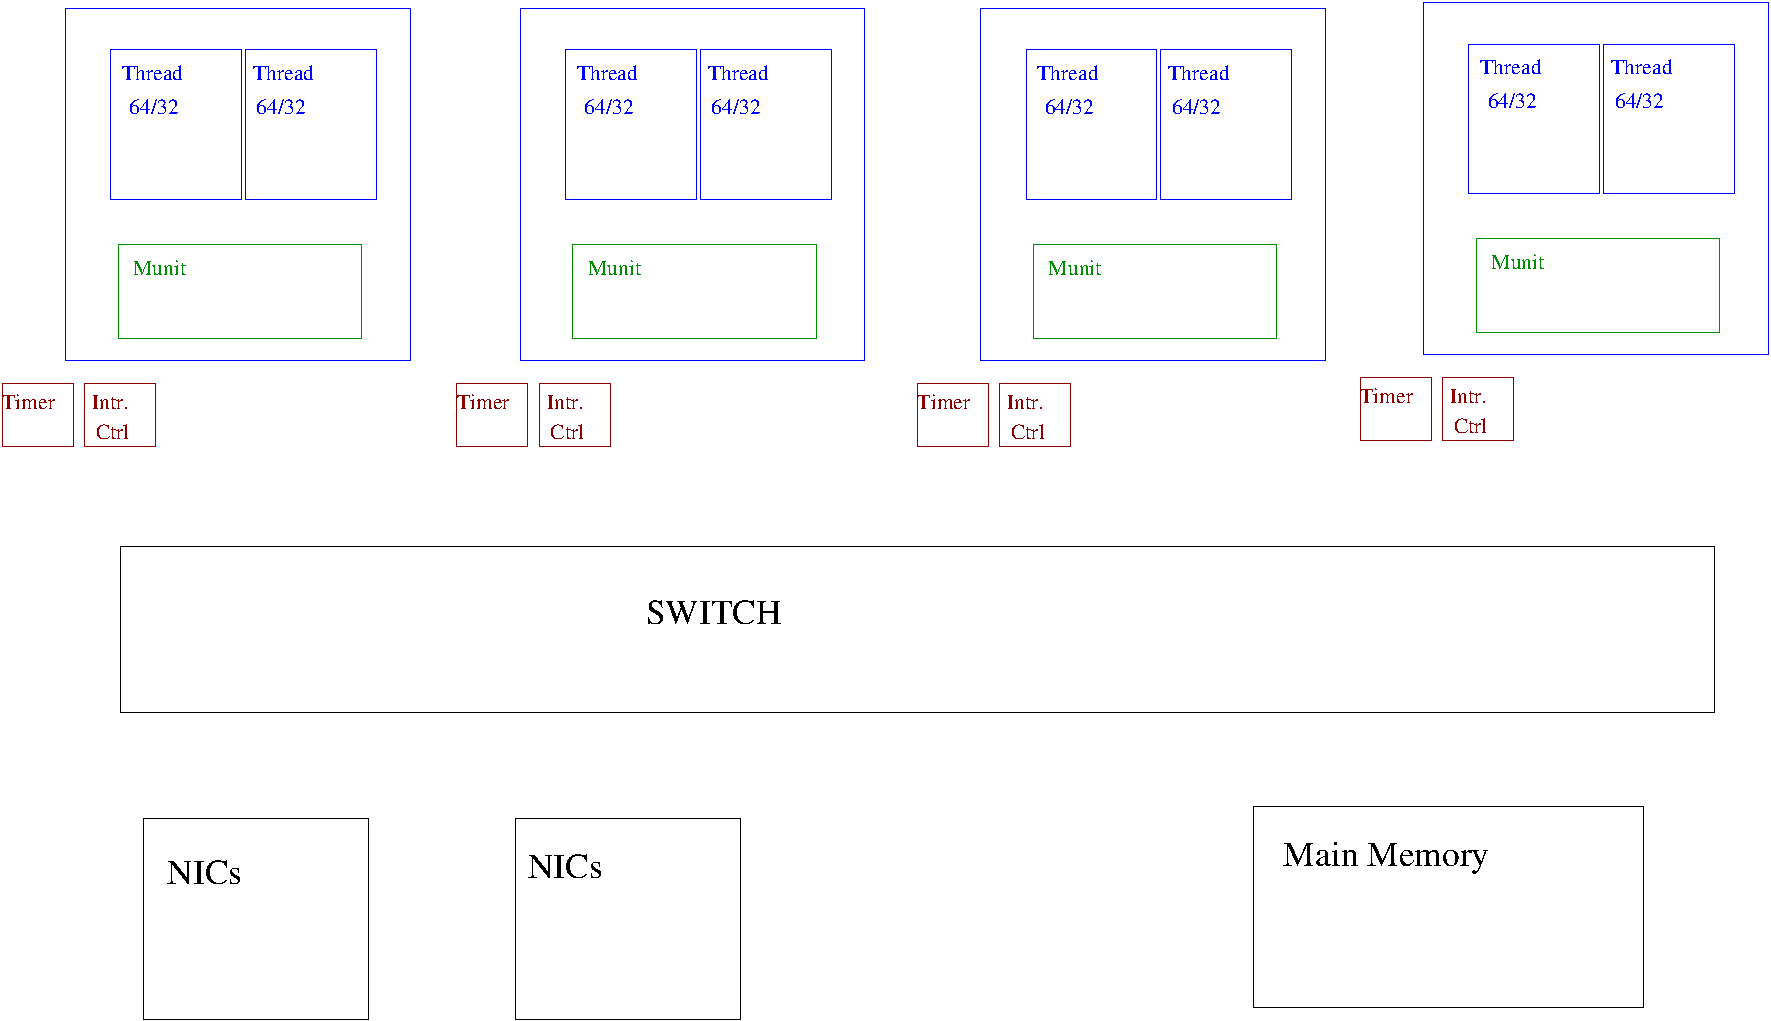
\includegraphics[width=10cm]{figs/Router_I.pdf}
  \caption{Router platform: phase 1}
  \label{fig:Phase1}
\end{figure}

The features of this platform are as follows:
\begin{itemize}
\item Vanilla NICs.
\begin{itemize}
\item NIC and main memory communicate directly.
\item NIC to NIC direct paths are provided.
\end{itemize}
\item Processor cores handle route lookup.
\item Software optimization.
\end{itemize}

\subsection{Phase 2}

\begin{figure}
  \centering
  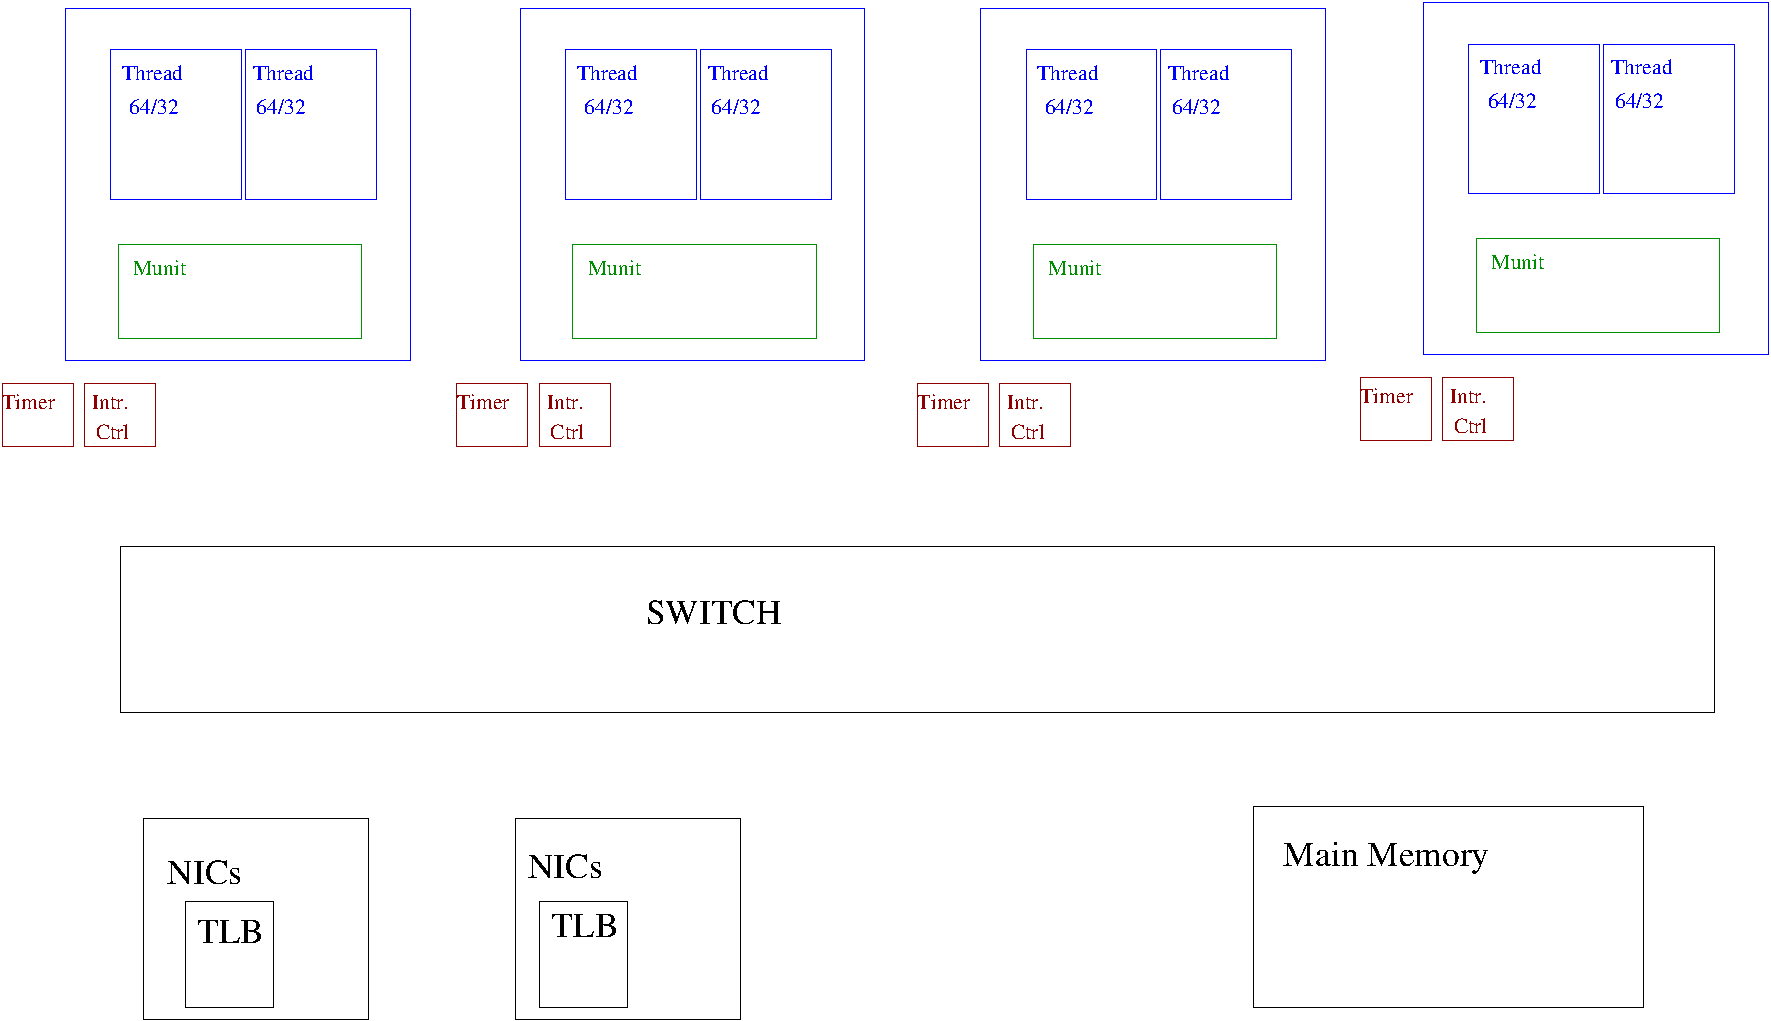
\includegraphics[width=10cm]{figs/Router_II.pdf}
  \caption{Router platform: phase 2}
  \label{fig:Phase2}
\end{figure}

In phase 2 (see Figure \ref{fig:Phase2}, 
the router will be enhanced with the following features:
\begin{itemize}
\item NICs with lookup caches.
\begin{itemize}
\item NIC and main memory communicate directly.
\item NIC to NIC communication is possible using
common switch.
\item On lookup cache hit, NIC to NIC packet
movement.
\item Packet modification in NIC.
\end{itemize}
\item Processor cores handle non-hit route lookups.
\end{itemize}
These enhancements aim at a 5X improvement over the Phase 1 router.

\subsection{Phase 3}
\begin{figure}
  \centering
  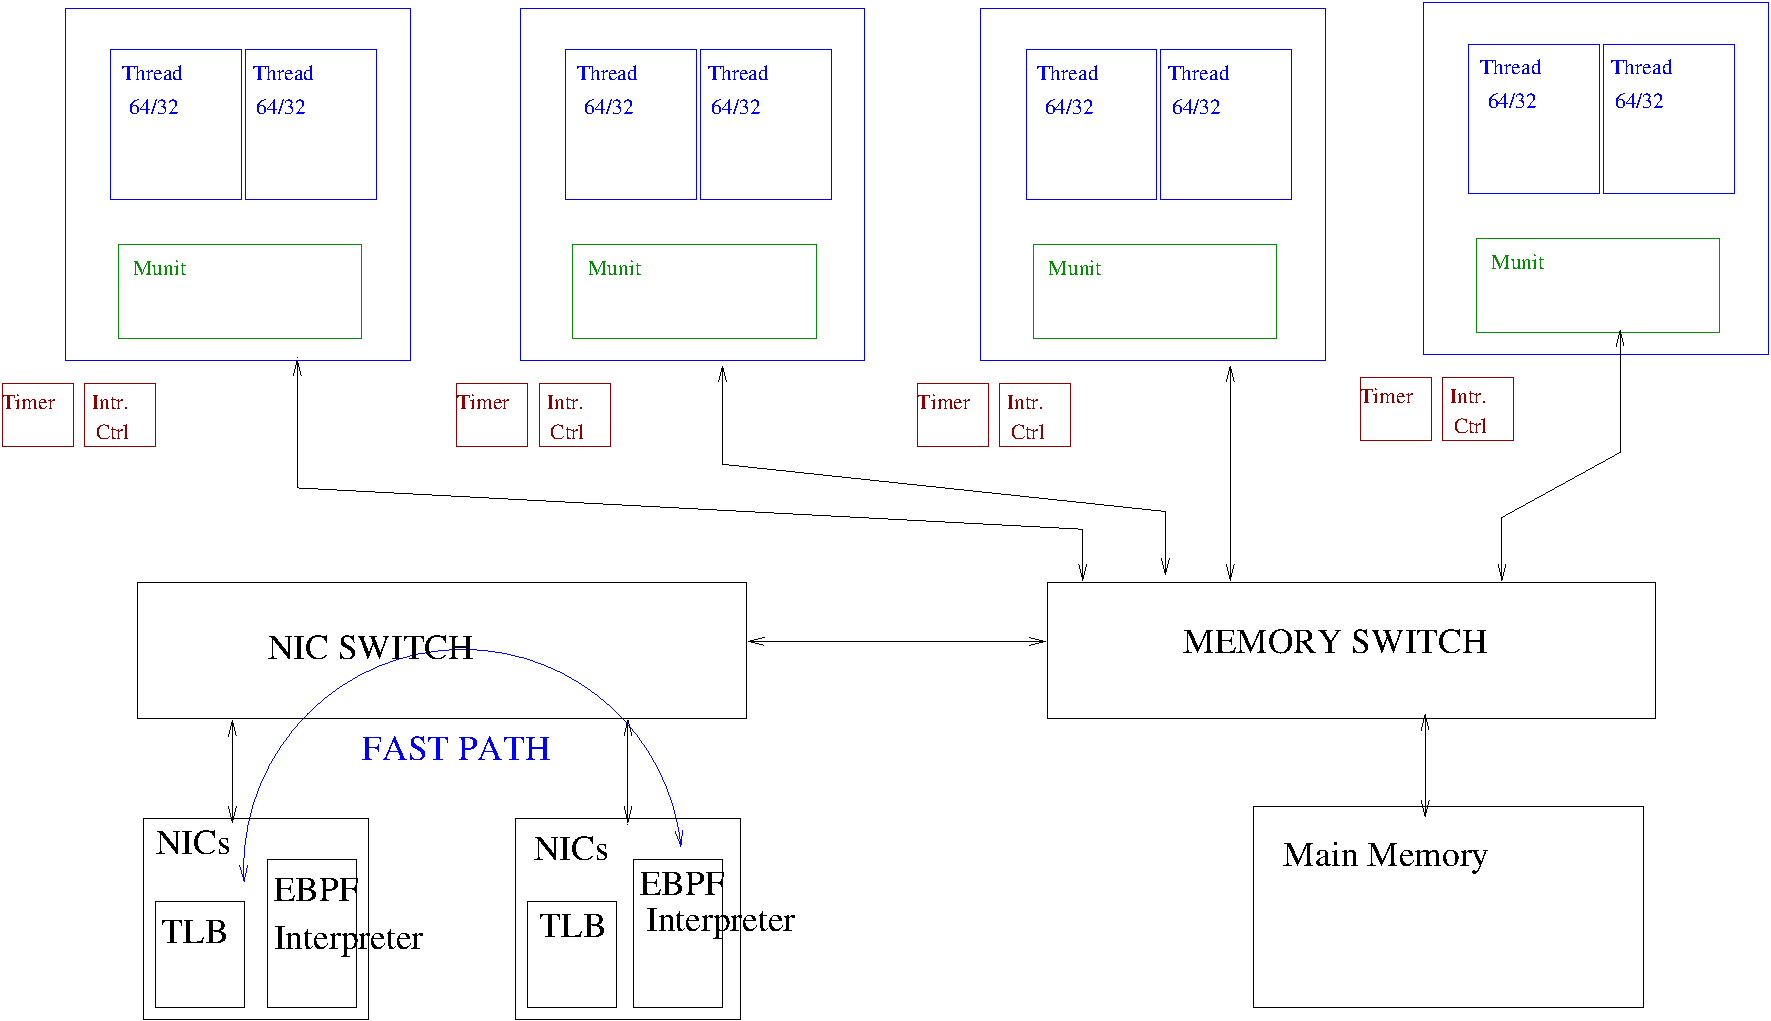
\includegraphics[width=10cm]{figs/Router_III.pdf}
  \caption{Router platform: phase 3}
   \label{fig:Phase3}
\end{figure}

In the phase 3 router, further enhancements will be
incorporated into the router platform.
\begin{itemize}
\item NICs with lookup caches and embedded EBPF interpreter.
\begin{itemize}
\item NIC and main memory communicate directly.
\item NIC to NIC high performance direct paths are provided via
separate switch.
\item Packet processing in NIC using EBPF interpreter.
\item On lookup cache or interpreter hit, NIC to NIC packet
movement.
\end{itemize}
\item Processor cores handle remaining route lookups.
\end{itemize}
As a result of these enhancements, we target a 5X performance
improvement over the Phase 2 router.

\subsection{Development process}

\begin{itemize}
\item Phase 1 (6 months):  port forwarding engine to 4-core 8-thread platform with vanilla NICs.
\item Phase 2 (6 months):  Control plane software port, add TLBs to NICs.
\item Phase 3 (6 months):  MPLS software port, add BPF interpreter to NICs.
\item On FPGA platform, demonstrate 1.6Gbps on Stage 1, 8 Gbps on Stage 2, 16 Gbps on Stage 3.
\item After FPGA validation, implement router ASIC (22nm, 1.2GHz, 10W).  Implementation will take 6-9 months.
\begin{itemize}
\item Target 100-200 Gbps in ASIC based router.
\end{itemize}
\end{itemize}

\section{Detailed Description of the project: software platform}

The software platform will be Release-15 compliant 5G Core for 
Private 5G Deployment, with support for
\begin{itemize}
\item User Plane Private 5G Network Functions: UPF  
\item IPv4, IPv6, MPLS and L3-VPN Forwarding.
\item Private 5G Control Plane functions: AMF, SMF, AUSF.
\item Routing Protocols like OSPF, ISIS, BGP, LDP
\end{itemize}

The software platform will be developed in two phases.

\subsection{Phase 1}

Integrate the User Plane of 5G Core and IP MPLS Router in the AJIT Hardware. 
At this point, the platform contains the 5G UPF and IP/ MPLS Packet Forwarding.

\subsection{Phase 2}

Integrate the Control Plane of 5G Core and IP MPLS Router in the AJIT Hardware. 
So, it contains the 5G control plane component such as SMF, AMF, AUSF, etc. and 
the IP/ MPLS Routing Protocols.

\subsection{Prototype deployment}

A prototype 5G router platform will be deployed on the FPGA platform of 
the hardware outlined above.  Use plane processing will be deployed as
part of phase 1, and control plane processing as part of phase 2.


\end{document}


